\lstset{style=TigerJython,escapeinside={(*@}{@*)}}
\fboxsep=.6pt

\newcounter{mycounter}\stepcounter{mycounter}
\iftoggle{teacherToggle}{
% initialize new counter for DLs and set it to 1


\section*{Begleitdokument für Lehrpersonen}
%\begin{itemize}
%    \item Einführung in den Semesterplan
%    \item Kontext (Voraussetzungen, Stufe, Empfehlung zur Einbettung und zur Fortsetzung)
%    \item Mögliche Schwierigkeiten der SuS und Lösungsvorschläge (für Gesamt-Programm)
%\end{itemize}

Dieses Dokument hat zum Ziel, einen Semester-Plan für die Einführung in das Programmieren auf Gymnasial-Stufe (Schweizer Bildungssystem, Sekundarstufe II, Altersstufe ca. 15-18 Jahre, obligatorisches Fach Informatik, kurz OInf) mittels Python zur Verfügung zu stellen. Das Semesterprogramm setzt keine besonderen Programmier- oder Informatikkenntnisse voraus. Das Semesterprogramm erstreckt sich über ca. 10 Lektionen und sollte den SuS ermöglichen, einfache mathematische und grafische Programme in Python zu schreiben. 

Da relativ wenig Zeit für das OInf zur Verfügung steht, liegt der Fokus dieses Semester-Programms auf grundlegenden Python-Kenntnissen. Als Fortsetzung und Vertiefung der neu gewonnen Kenntnisse empfiehlt sich eine Einführung in die Robotik im OInf, beziehungsweise eine Vertiefung der Programmierung im Ergänzungsfach, beispielsweise mit Themen wie Rekursion oder objektorientierter Programmierung (in Python).

Beim untenstehenden Themenüberblick wurde insbesondere darauf geachtet, die Reihenfolge möglichst sinnvoll zu gestalten, so dass die Kenntnisse schrittweise erweitert und aufeinander aufgebaut werden können. Zudem wurde darauf geachtet, stets ein möglichst ausgeglichenes Verhältnis zwischen ``theoretisch-mathematischen'' und ``grafisch-interaktiven'' Aufgaben zu bewahren (da letztere die SuS erfahrungsgemäss stärker motivieren).

\begin{overviewBox}[title=Überblick der Themen]
    \begin{enumerate}
    \item \textbf{Allgemeine Motivation und Einführung ins Programmieren}
    \begin{itemize}
        \item 1-2 Beispiele mit Bezug zur Lebenswelt und Vorwissen von SuS, einige Algorithmen und Beispiele zu logischem Denken
        \item Vordefinierte Grafik-Befehle mit \lstinline|turtle| (nur ein Parameter): \lstinline|forward()|, \lstinline|right()|
        \item Einfache Schleifen mit \lstinline|for i in range(...)|
    \end{itemize}
    \item \textbf{Datentypen und Syntax}
    \begin{itemize}
        \item Variablen und Zuweisung vs. Mathematik
        \item Arbeiten mit einfachen mathematischen Operatoren
        \item Arbeiten mit Text
        \item Debugging-Übungen (syntax vs. runtime vs. semantic errors), typische Fehler
    \end{itemize}
    \item \textbf{Verzweigungen} (\lstinline|if...elif...else|) \& \lstinline|while|,  elementare logische Operatoren (or, and, xor)  und Flussdiagramme
    \item \textbf{Befehle / Funktionen} (\lstinline|def|)
    \begin{itemize}
        \item Ohne Parameter, ohne \lstinline|return|
        \item Mit Parameter, ohne \lstinline|return|
        \item Mit Parameter, mit \lstinline|return|
    \end{itemize}
    \item \textbf{Listen}
    \begin{itemize}
        \item  Koordinatengrafik, Zufallszahlen, \lstinline|random|-Library ($\rightarrow$ \lstinline|turtle|), \item Schleifen / Traversieren (\lstinline|for item in mylist|)
    \end{itemize}
\end{enumerate}
\end{overviewBox}


Mögliche Schwierigkeiten, die Auftreten können:
\begin{enumerate}
\item \textbf{Zeitbedarf}: Übungen zu neuen Teilen können erfahrungsgemäss viel Zeit beanspruchen, insbesondere Übungen zu Syntax oder Funktionen. Dabei kann es hilfreich sein, die Übungen von Anfang an mit einer Zeiteinschätzung zu versehen und einzuplanen, welche Übungen bei Bedarf gestrichen, beziehungsweise auf eine andere Lektion verschoben, oder als Challenge-Aufgabe für Schnelle deklariert werden sollen.
\item \textbf{Abstraktes Denken}: Gerade in Bereichen wie Verzweigungen und Flussdiagrammen, oder beim Traversieren von Listen, zeigt sich, dass das abstrakte Denken --- insbesondere in tieferen Altersstufen --- häufig noch nicht ausreichend entwickelt ist. Daher kann es, sofern diese Möglichkeit besteht, sinnvoll sein, das Semesterprogramm erst in einem späteren Semester auszuführen.
\item \textbf{Technische Probleme}: \textit{Shortcuts}, Programme installieren, Programme abspeichern --- all dies ist für viele SuS entgegen der Erwartung vieler LP noch neu. Dazu kommen häufige Probleme beim Betreiben eigener Geräte (BYOD). Daher sollte genügend Zeit eingeplant werden, um auch auf solche Faktoren einzugehen und um ``softes'' Wissen zu vermitteln.
\end{enumerate}

\clearpage
}{}

\tableofcontents
\clearpage
\section*{Installation von Python und VSCodium}
Um mit dem Programmieren loslegen zu können, müssen wir zuerst die Programmiersprache auf unserem Computer installieren, sowie ein Programm, mit welchem wir Python-Code schreiben und ausführen können. Ein solches Programm wird typischerweise \gls{IDE} genannt. In diesem Skript verwenden wir die kostenfreie Programmiersprache Python, sowie die ebenfalls kostenfreie, weit verbreitete \gls{IDE} VSCodium. Der nachfolgende Abschnitte leitet Sie durch die Installation sowohl auf Windows wie auf MacOS.

\subsection*{Installation von Python}
...

\subsection*{Installation von VSCodium}
...

\section{DL \themycounter: Allgemeine Motivation und Einstieg ins Programmieren}
\iftoggle{teacherToggle}{
\begin{myExBox}[title=DL \themycounter]
\tcbsubtitle{Thema}
Die Lektion soll den Einstieg in die (für die meisten SuS noch neue) Welt des Programmierens machen. Dabei werden zuerst das Thema ``Programmieren'' im Allgemeinen und danach Python als spezifische Programmiersprache für diesen Semester-Kurs vorgestellt. Abschliessend führen einige einfache grafische Beispiele mit der \lstinline|turtle|-Library die SuS an die Programmierung mit Python heran.


\tcbsubtitle{Operationalisierte Lernziele}
\begin{todolist}
    \item Die SuS können Beispiele aus ihrem eigenen Alltag nennen, wo Algorithmen eine Rolle spielen.
    \item Die SuS können logische Prozesse aus der ihnen bekannten Alltagswelt mithilfe von Flussdiagrammen modellieren.
    \item Die SuS können grundlegende \lstinline|turtle|-Befehle wie \lstinline|forward()|, \lstinline|right()| und \lstinline|left()| ausführen, um damit einfache Zeichnungen zu erstellen.
    \item Die SuS können einfache Formen mit einer \lstinline|for i in range(start, end, step)|-Schleife zeichnen, beispielsweise ein Quadrat oder ein Sechs-Eck.
\end{todolist}

\tcbsubtitle{Grober Lektionsablauf}
\textbf{Lektion 1/2: Programmieren \& Algorithmen}

Erste Hälfte der Lektion: Die SuS werden an das Thema Programmieren herangeführt und lernen dessen Relevanz anhand einiger alltagsnaher Beispiele kennen: Messgeräte in Spitäler (unterliegende Idee: \lstinline|if...elif...else|), Sensoren in Autos (z.B. \lstinline|while|), etc. Dabei lernen die SuS, die unterliegenden Algorithmen als Flussdiagramme darzustellen. Zweite Hälfte: Die SuS lösen eigenhändig Übungen und wenden ihr neu gewonnenes Wissen zu Flussdiagrammen auf die Übungen an (Abgabe auf Moodle).

\textbf{Lektion 2/2: Programmieren mit Python und \lstinline|turtle|}

Die SuS lernen Python kennen und installieren ein lokales IDE. Danach führen sie, geleitet durch die LP, einige Übungen durch, um einfache Formen mit der Schildkröte zu zeichnen. Dabei lernen Sie die erste einfache Schleife (\lstinline|for i in range(start, end, step)|) kennen.

\begin{myExBox}[title=Mögliche Schwierigkeiten \& geeignete Massnahmen]
\begin{enumerate}
    \item Abstraktes Denken zu Flussdiagrammen ist komplex und herausfordernd. Der wäre es hilfreich, bereits zu Beginn des Unterrichts ein Nachschlagewerk zur Verfügung zu stellen, welches die SuS dabei unterstützt, die Übungen zu lösen, indem sie bei Bedarf nachlesen können.
    \item BYOD als Herausforderung: Möglicherweise gestaltet sich der Installationsprozess komplexer und langwieriger als gedacht. Daher sollte die Installation des IDE nach Möglichkeit bereits im Voraus als Hausaufgabe (mittels Schritt-für-Schritt-Dokumentation) ausgeführt worden sein.
    \item Technische Herausforderungen beim Ausführen von Code: Gerade in der ersten Lektion brauchen einige SuS noch Unterstützung beim Ausführen und Debuggen von Code (``wo ist der Run-Knopf?''). Mögliche Lösungsansätze könnten sein, genügend Zeit für die Übungen einzuplanen (s. Punkt 2), bzw. den Einstieg nach Möglichkeit in Halbklassen zu machen. 
\end{enumerate}
\end{myExBox}
\end{myExBox}
\newpage}{}
\stepcounter{mycounter}

\section{DL \themycounter: Datentypen und Syntax (Variablen \& Zahlen)}
\iftoggle{teacherToggle}{
\begin{myExBox}[title=DL \themycounter]
\tcbsubtitle{Thema}
In dieser Doppellektion geht es darum, die SuS an die Grundlagen von Datentypen sowie einige grundlegende syntaktische Elemente in Python heranzuführen. Dabei soll, in der ersten der beiden dafür vorgesehenen Doppellektionen, der Fokus auf mathematische Operationen gelegt werden, wodurch die SuS hoffentlich auch einen Bezug zu ihrem Vorwissen herstellen können.

\tcbsubtitle{Operationalisierte Lernziele}
\begin{todolist}
    \item Die SuS können das Gleichzeichen verwenden, um Variablen zu erstellen. Sie können in eigenen Worten erklären, was der Unterschied zwischen dem Gleichzeichen in Python und dem Gleichzeichen in der Mathematik ist.
    \item Die SuS können einfache Rechnungen machen, indem Sie Variablen erstellen und einfache mathematische Operatoren verwenden.
    \item Die SuS können den Inhalt einer Variable \lstinline|x| mit \lstinline|print(x)| ausgeben.
    \item Die SuS können den Modulo-Operator (\texttt{\%}) korrekt verwenden, beispielsweise um alle geraden Zahlen in einer Schleife auszugeben  (s. DL 1 für einfache Schleifen).
    \item Die SuS können Weret einer Variable in einer Schleife verändern, indem Sie \textit{compound operators} wie beispielsweise \lstinline|+=|, \lstinline|-=|, \lstinline|*=| oder \lstinline|/=| verwenden.
    \item Die SuS können Funktionen, um die Wurzel einer Zahl (z.B. \lstinline|sqrt(x)|) oder deren Quadrat (z.B. \lstinline|x**2|) sinnvoll verwenden und das Resultat in einer Variable speichern sowie ausgeben.
    \item Die SuS können einfache Formen mit Pythagoras zeichnen (beispielsweise ein schräges Dach in einem Haus)
    \item Die SuS können Probleme aus der Mathematik, wie beispielsweise polynomiale Gleichungen, mit einem Python-Code implementieren und lösen.
\end{todolist}

\tcbsubtitle{Grober Lektionsablauf}
\textbf{Lektion 1/2: Einführung und Übungen}

Alltagsnahe Beispiele werden aufgezeigt, um das Interesse für mathematische Operatoren zu wecken. Man könnte beispielsweise aufzeigen, wie aus einer Liste von Körpergrössen diejenige ausgeben kann, deren Körpergrösse eine gerade Zahle ist. Da die Doppellektion eher voll beladen ist, wird diese Sequenz jedoch relativ kurz gehalten, um genug Zeit für die Übungen zu lassen. Die Übungen sind, wie immer, im Skript, und die Erklärungen zu den neuen Konzepten, welche mit dem einführenden Beispiel vermittelt wurden, können dort bei Bedarf nochmals nachgelesen werden.

\textbf{Lektion 2/2: Übungen}

Lektion 2 widmet sich hauptsächlich den Übungen. Am Schluss wird, je nach dem welche Schwierigkeiten bei den SuS während den Übungen beobachtet wurde, nochmals auf einige herausfordernde Aufgaben eingegangen, und danach wird eine Ergebnissicherung (neue Konzepte) durchgeführt.

\begin{myExBox}[title=Mögliche Schwierigkeiten \& geeignete Massnahmen]
\begin{enumerate}
    \item Die SuS könnten verwirrt sein, weshalb mit dem Gleichzeichen nun etwas anderes gemeint ist als in der Mathematik (Zuweisung statt Gleichheit). Dies könnte durch klare grafische Darstellungen gelöst werden, etwa wie folgt: $  \tikzmarknode{b}{\text{\texttt{a}}} =\tikzmarknode{a}{\color{red}\underbrace{\color{black}\text{\texttt{10+3}}}}
        $
    \tikz[remember picture, overlay]{\draw[-latex,red] ([yshift=0.1em]a.south) to[bend left] ([yshift=-0.3em]b.south);}
	Die Erklärung dazu könnte lauten: ``Wir werten \lstinline|10+3 = 13| aus und speichern den Wert \lstinline|13| in der Variable \lstinline|a|''.
	\item Die Lektion könnte zu kurz sein für alle Inhalte. Allenfalls müsste nach einer ersten Durchführung entschieden werden, ob Teile der Lektion in DL 3 durchgeführt werden, welche aus diesem Grund weniger umfangreich geplant ist.
\end{enumerate}
\end{myExBox}
\end{myExBox}
\newpage\stepcounter{mycounter}}

\section{DL \themycounter: Datentypen und Syntax (Text \& Debugging)}
\begin{myExBox}[title=DL \themycounter]
\tcbsubtitle{Thema}
In dieser zweiten, den Datentypen und Grundlagen sowie der Syntax gewidmeten Doppellektion geht es darum, elementare Text-Operationen kennenzulernen und diese sinnvoll zu verwenden. Ebenfalls soll sichergestellt werden, dass die SuS geläufige Laufzeit-Probleme aufgrund von Datentypen selbstständig entdecken und beheben können.


\tcbsubtitle{Operationalisierte Lernziele}
\begin{todolist}
    \item Die SuS können in eigenen Worten beschreiben, was eine Zeichenkette in Python ist, und können eine solche selbstständig erstellen.
    \item Die SuS können Zeichenketten mit \lstinline|"..." + "..."| verketten.
%    \item Die SuS können Zeichenketten mit \lstinline|"..." * [zahl]| beliebig viele Male wiederholen.
%    \item Die SuS können mithilfe von Spezialzeichen (z.B. \lstinline|\n|) sowie \lstinline|print()| einfache ASCII-Zeichnungen machen, wie etwa einen Pfeil.
%    \item Die SuS können Zeichenketten sowohl innerhalb einfacher wie doppelter Klammern (\lstinline|'...'| oder \lstinline|"..."|) schreiben, den Unterschied zwischen den beiden in eigenen Worten erklären und diesen Unterschied anhand eines Beispiels veranschaulichen (z.B. \lstinline|print('Meine Freunde nennen mich "Mr. X"')|).
%    \item Die SuS können geläufige Laufzeit-Probleme wie etwa die nicht funktionalen Ausdrück \lstinline|print("1+2")| oder \lstinline|print(Hallo Welt)| als solche erkennen und beheben.
%    \item Die SuS können die Funktion \lstinline|input("Fragetext")| verwenden, um einen Wert (Text oder Zahl) während der Laufzeit zu generieren. Diesen können die SuS in einer Variable abspeichern und weiterverwenden.
\end{todolist}

%\tcbsubtitle{Grober Lektionsablauf}
%
%Ähnlich wie die vorherige Doppellektion, beginnt auch diese Doppellektion mit einigen alltagsnahen Beispielen, die direkt im Code-Editor vorgezeigt und ausgeführt werden. Beispielsweise könnte mit \lstinline|input| nach einem Namen gefragt werden, der dann in der Konsole 20 mal als ASCII-Zeichnung ausgegeben wird. Nach einer relativ kurzen Einführungssequenz wird der Rest der Doppellektion den Übungen sowie einer Ergebnissicherung gewidmet, wobei letztere insbesondere nochmals Debugging-relavante Aufgaben aufgreift (welche im Skript an letzter Stelle dieser Doppellektion vorkommen).
%
%\begin{myExBox}[title=Mögliche Schwierigkeiten \& geeignete Massnahmen]
%\begin{enumerate}
%    \item Die SuS könnten unter Umständen verwirrt sein, weshalb \lstinline|turtle|-Grafiken in einem separaten Fenster gezeichnet werden, währenddem der \lstinline|print()|-Befehl in der Konsole ausgegeben wird. Darauf sollte in der Einführung eingegangen werden.
%    \item Die SuS könnten Mühe haben mit dem Abstraktionsgrad von Zeichenketten (Wiederholungen etc.) und durch die Syntax verwirrt sein (beispielsweise die Möglichkeit, Zeichenketten mit einem einfachen oder doppelten Anführungszeichen zu schreiben). Diesen Aspekten sollte daher sowohl während der Präsentation wie auch im Skript besondere Aufmerksamkeit gewidmet werden.
%\end{enumerate}
%\end{myExBox}
\end{myExBox}


\subsection{Zeichenketten in Python}
Im Nachfolgenden schauen wir uns einige Python-Befehle an, die dazu dienen, mit Zeichenketten (=engl. \textit{strings}) zu arbeiten. Dies werden wir insbesondere benötigen, um eigene Python-Programme zu schreiben, mit denen wir Texte verschlüsseln und entschlüsseln können. Genauer gesagt bezeichnen wir Texte in Python als Zeichenketten. Zeichenketten werden in Python innerhalb von einfachen oder doppelten Anführungszeichen geschrieben, also entweder \lstinline|'...'| oder \lstinline|"..."|. Innerhalb der Anführungszeichen können beliebige Zeichen stehen, beispielsweise Buchstaben, Leerzeichen, Spezialzeichen oder Zahlen.

\begin{mychallenge}
Was könnte der Nutzen davon sein, dass es zwei Möglichkeiten gibt und nicht nur eine, Zeichenketten zu schreiben (\lstinline|'...'| oder \lstinline|"..."|)? 
\begin{myanswer}
Eine Möglichkeit, die uns durch die unterschiedlichen Schreibweisen geboten wird, ist, Anführungszeichen auszugeben. Beispielsweise könnten Sie so einen Text, der Anführungszeichen beinhaltet, auf der Konsole drucken:
\begin{lstlisting}
print('Meine Freunde nennen mich "Mr. X"')
\end{lstlisting}
\end{myanswer}
\end{mychallenge}

Mit der \textbf{Länge} von Zeichenketten ist die Anzahl der Zeichen zwischen den Anführungszeichen gemeint: Die Zeichenkette \lstinline|"Hello World"| hat beispielsweise eine Länge von 11 Zeichen. Die Länge einer Zeichenkette kann mit dem Ausdruck \lstinline|len(Klartext)| bestimmt werden.

\begin{myexercise}
Bestimmen Sie die Länge Ihres vollen Namens mithilfe des Befehls \lstinline|len()| in Python.
\end{myexercise}

Zeichenketten können verkettet, also aneinandergehängt werden mit dem Befehl \lstinline|"Text1" + "Text2" + "Text3"| usw. Falls Sie eine Zeichenkette mehrfach drucken wollen, können Sie diesen mit einer Zahl multiplizieren, die dann die Anzahl Wiederholungen der Zeichenkette bestimmt. So ist der Ausdruck \lstinline|"a" * 3| beispielsweise gleichbedeutend mit einer Zeichenkette \lstinline|"aaa"|.

\begin{myexercise}\label{ex:pfeil}
Führen Sie das nachfolgende Programm aus und erklären Sie, was das Programm tut.
  \begin{lstlisting}
    print(" " * 3 + "X" * 1)
    print(" " * 2 + "X" * 3)
    print(" " * 1 + "X" * 5)
    print(" " * 0 + "X" * 7)
    print(" " * 3 + "X" * 1)
    print(" " * 3 + "X" * 1)
  \end{lstlisting}
\end{myexercise}


\begin{myexercise}
Erstellen Sie nun ein Programm, das ein Herz zeichnet, ähnlich zu \cref{ex:pfeil}, also lediglich mit Zeichenketten-Ausdrücken und dem Befehl \lstinline|print()|.
\begin{myanswer}
\begin{lstlisting}
print(" " * 2 + "X" * 1 + " "*4+"X" * 1 + " "*1)
print(" " * 1 + "X" * 8 + " "*1)
print(" " * 2 + "X" * 6 + " "*1)
print(" " * 3 + "X" * 4 + " "*2)
print(" " * 4 + "X" * 2 + " "*2)
\end{lstlisting}
\end{myanswer}
\end{myexercise}

\begin{myexercise}\label{ex:name}
Schreiben Sie ein Programm, das Sie nach Ihrem Namen fragt. Danach soll Sie das Programm neun Mal begrüssen, indem es auf 3 Zeilen je dreimal den Text ``\texttt{Hallo [Ihr Name]}'' druckt.
\begin{myanswer}
  \begin{lstlisting}
	name = input("Wie heissen Sie?")
	
	repeat 3:
	    print(("Hallo " + name + " ")*3)
  \end{lstlisting}
\end{myanswer}
\end{myexercise}


\subsection{Zeichen aus Zeichenketten auslesen}
Im Nachfolgenden schauen wir uns einige Übungen an, mit denen wir die einzelnen Zeichen aus Zeichenketten herauslesen können.

\begin{myexercise}
  Führen Sie das nachfolgende Programm aus und erklären Sie, was das Programm tut.
  \begin{lstlisting}
    text = "EASY"
    for buchstabe in text:
      print(buchstabe)
  \end{lstlisting}
  \begin{myanswer}
    \begin{lstlisting}
      E
      A
      S
      Y
    \end{lstlisting}
    \pythoninline{for x in mystring} ist eine Schleife über die Zeichenkette \pythoninline{mystring}. Dabei nimmt \pythoninline{x} nacheinander jeden Buchstaben in dieser Zeichenkette genau einmal an.
  \end{myanswer}
\end{myexercise}

\begin{myexercise}\label{myexercise:index}
  Führen Sie das nachfolgende Programm aus und erklären Sie, was das Programm tut.
  \begin{lstlisting}
    Klartext = "Schweiz"
    print(Klartext[0])
    print(Klartext[1])
    print(Klartext[2])
    print(Klartext[3])
    print(Klartext[4])
    print(Klartext[5])
    print(Klartext[6])
  \end{lstlisting}
  \begin{myanswer}
    \begin{lstlisting}
      S
      c
      h
      w
      e
      i
      z
    \end{lstlisting}
    \pythoninline{mystring[0]} ist der erste Buchstabe der Zeichenkette \pythoninline{mystring}, \pythoninline{mystring[1]} der zweite und so weiter.
  \end{myanswer}
\end{myexercise}

\begin{myexercise}
  Führen Sie das nachfolgende Programm aus und erklären Sie, was das Programm tut.
  \begin{lstlisting}
    Klartext = "Schweiz"
    for i in range(len(Klartext)):
      print(Klartext[i])
  \end{lstlisting}
  \begin{myanswer}
    Dieses Programm ist äquivalent zum Programm in \cref{myexercise:index}. 
    Hier wird allerdings eine \pythoninline{for}-Schleife über die Länge des Texts verwendet.
  \end{myanswer}
\end{myexercise}

Der Befehl \lstinline|for i in range(len(Klartext))| erstellt eine Variable \lstinline|i| innerhalb der \lstinline|for|-Schleife, welche jedes Zeichen von 0 bis zur Länge von \lstinline|Klartext| minus 1 geht. Weshalb minus 1? Das erste Zeichen von \lstinline|Klartext| wird in Python mit \lstinline|Klartext[0]| ausgelesen, das letzte mit \lstinline|Klartext[len(Klartext)-1]|, da wir bei 0 zu zählen beginnen und nicht bei 1. Mit dem Ausdruck \lstinline|Klartext[i]| wird also das \lstinline|i|-te Zeichen der Zeichenkette \lstinline|Klartext| ausgelesen, wobei \lstinline|i| von 0 bis zu (Länge des Klartexts minus 1) geht. 

Der Befehl \lstinline|for i in range(len(Klartext))| kann auch geschrieben werden also Befehl \lstinline|for i in range(0, len(Klartext), 1)|, wobei dies meint:
\begin{itemize}
\item \lstinline|i| beginnt bei 0
\item \lstinline|i| geht bis zu \lstinline|len(Klartext)-1|
\item \lstinline|i| vergrössert sich in 1er-Schritten
\end{itemize}
Dieser Befehl könnte auch verwendet werden, um bei einer beliebigen Zahl zu starten (nicht notwendigerweise 0), und um \lstinline|i| in Schritten grösser als 1 zu vergrössern. Die allgemeine Syntax des Befehls lässt sich also wie folgt zusammenfassen: \lstinline|for i in range(start, ende, schrittgroesse)|.

\begin{mychallenge}
  Eine Person verrät uns lediglich die Vorwahl ihrer $10$-stelligen Mobiltelefonnummer. Zudem verrät Sie Ihnen auch, dass ihre Telefonnummer gerade ist (also auf 2, 4, 6, 8 oder 0 endet).
  Damit gibt es nur noch $5$ Millionen Kombinationen, die es (im schlimmsten Fall) auszuprobieren gilt. 
  Schreiben Sie ein Python-Programm, welches die $2000$ kleinsten, geraden Nummern auflistet. 
  Die erste Nummer sollte $0790000000$ sein, die letzte $0790001999$. 
  Das Programm soll die Nummern als Zeichenkette (eine Nummer pro Zeile) ausgeben.
  
  Tipps:
  \begin{itemize}
    \item Mit \pythoninline{str(num)} 
      wird aus der Zahl \pythoninline{num} eine Zeichenkette.
      Beispielsweise gibt uns \pythoninline{str(15)}
      die Zeichenkette \lstinline[language=Python,basicstyle=\ttfamily\normalsize]!"15"!.
    \item Erinnern Sie sich, was die Operation \pythoninline{+} in dem Ausdruck \lstinline[language=Python,basicstyle=\ttfamily\normalsize]!"In" + "form" + "atik"! macht?
  \end{itemize}
  \begin{myanswer}
    \begin{lstlisting}
      for num in range(790000000, 790002000,2):
        print("0" + str(num)) # füge die Zeichenkette "0" vorne an
    \end{lstlisting}
  \end{myanswer}
\end{mychallenge}

\newpage\stepcounter{mycounter}



\section{DL \themycounter: Verzweigungen mit \texorpdfstring{\lstinline|if...elif...else|}{if...elif...else}}
\begin{myExBox}[title=DL \themycounter]
\tcbsubtitle{Thema}
Die SuS lernen das Programmieren mit konditionaler Logik kennen, indem Sie mit den Befehlen \lstinline|if|, \lstinline|elif| und \lstinline|else| vertraut gemacht werden. Dabei wird nochmals das in DL 1 angeeignete Wissen zu Flussdiagrammen aufgefrischt, um die neuen Konzepte grafisch (im Sinne der \textit{dual-code}-Theorie) zu unterstützen und aufzuwerten.

\tcbsubtitle{Operationalisierte Lernziele}
\begin{todolist}
    \item Die SuS können in ihrem Programm konditionale Logik implementieren, indem sie die Befehle \lstinline|if|, \lstinline|elif| und \lstinline|else| verwenden.
    \item Die SuS verstehen die Bedeutung der Einrückung in Python.
    \item Die SuS können einen gegebenen Code als Flussdiagramm veranschaulichen.
    \item Die SuS können erklären, weshalb ein bestimmter Code (nicht) ausgeführt wird.
    \item Die SuS können in ihrem Programm logische Tests implementieren. Dabei können Sie die Operatoren \lstinline|!=|, \lstinline|<|, \lstinline|<=|, \lstinline|>=|, \lstinline|>| und \lstinline|==| korrekt auf Zahlen- sowie Text-Variablen anwenden.
    \item Die SuS können logische Tests korrekt negieren, indem sie den Operatoren \lstinline|not| verwenden.
    \item Die SuS können zwischen der Negation und dem Gegenteil einer (logischen) Aussage unterscheiden, indem sie deren Unterschied anhand von Alltagsbeispielen aufzeigen
\end{todolist}

\tcbsubtitle{Grober Lektionsablauf}
Ähnlich wie die vorherigen Doppellektionen beginnt auch diese Doppellektion mit einigen alltagsnahen Beispielen, die direkt im Code-Editor vorgezeigt und ausgeführt werden. Dabei wird parallel zum Code ebenfalls eine Visualisierung des Codes als Flussdiagramm gezeigt, wie folgt:\\[-.2cm]
\begin{minipage}[H]{.45\textwidth}
\begin{lstlisting}[basicstyle=\ttfamily\small]
note = input("Benoten Sie die Lehrperson (0-100).")
if note == 100:
    print("Vielen Dank! :)")
elif note > 60:
    print("Wie kann ich mich verbessern?")
else:
    print("Geben Sie mir eine Chance!")
\end{lstlisting}
\end{minipage}
\begin{minipage}[H]{.55\textwidth}
\begin{figure}[H]
\centering
\begin{tikzpicture}[node distance=2.5cm, scale=.5, transform shape, on grid, ->]
    \tikzstyle{every node}=[font=\small]
    % grid to easier see that the node centers line up while developing plot
    %\draw [help lines] (-5,-9) grid (9,1);
    \node (start) [code] {\pythoninline{note = input("Benoten Sie die Lehrperson")}};
    \node (dec1) [decision, below of=start] {\pythoninline{note == 100}};
    \node (printif) [code, text width=7cm, right=7cm of dec1] {\pythoninline{print("Vielen Dank! :)")}};
    \node (dec2) [decision, below of=dec1] {\pythoninline{note > 60}};
    \node (printelif) [code, text width=7cm, right=7cm of dec2] {\pythoninline{print("Wie kann ich mich verbessern?")}};
    \node (printelse) [code, text width=6cm, below of=dec2] {\pythoninline{print("Geben Sie mir eine Chance!")}};
    \node (end) [circle,draw=black, fill=black, below of=printelse, yshift=.5cm] {};
    
    \draw (start) -- (dec1);
    \draw (dec1) -- node[anchor=top, above=.1cm] {\pythoninline{True}} (printif);
    \draw (dec1) -- node[anchor=east] {\pythoninline{False}} (dec2);
    
    \draw (dec2) -- node[anchor=top, above=.1cm] {\pythoninline{True}} (printelif);
    \draw (dec2) -- node[anchor=east] {\pythoninline{False}} (printelse);
    
    \draw (printif) --++ (4.5cm,0cm) |- (end);
    \draw (printelif) --++ (4.5cm,0cm) |- (end);
    
    \draw (printelse) -- (end);
    
\end{tikzpicture}
\end{figure}
\end{minipage}
Das Beispiel würde aber Schritt für Schritt eingeführt, um den Unterschied zwischen folgenden drei Dingen klar aufzuzeigen: \begin{enumerate*}
\item \lstinline|if| \textit{ohne} \lstinline|elif| und \textit{ohne} \lstinline|else| 
\item \lstinline|if| \textit{ohne} \lstinline|elif| aber \textit{mit} \lstinline|else| 
\item \lstinline|if| \textit{mit} \lstinline|elif| und \textit{mit} \lstinline|else|
\end{enumerate*}. Ebenfalls können weitere alltagsnahe Beispiele (zumindest konzeptuell) aufgezeigt werden, um klarzustellen, wozu die konditionale Logik dienen kann (medizinische Bereiche, selbstfahrende Autos etc.). Danach üben die SuS das neu gewonnene Wissen, indem Sie es auf Zeichenketten, Texte und mit \lstinline|turtle| anwenden. Am Schluss findet wie immer eine Ergebnissicherung statt.

\begin{myExBox}[title=Mögliche Schwierigkeiten \& geeignete Massnahmen]
\begin{enumerate}
    \item Die SuS finden es schwierig zu erkennen, ob Code nach einem \lstinline|elif| oder \lstinline|else| noch ausgeführt wird, da sie nicht verstehen, dass diese Blöcke nur dann ausgeführt werden, wenn vorher das \lstinline|if| \lstinline|False| war. Im Unterricht sollten daher einige Beispiele aufgezeigt werden, die dies veranschaulichen
    \item Die Negation einer Aussage ist nicht dasselbe wie deren Gegenteil. Dies sollte anhand von alltagsnahen Beispielen (z.B. der Aussage ``der Schrank ist voll'') aufgezeigt werden.
 \end{enumerate}
\end{myExBox}
\end{myExBox}
\newpage\stepcounter{mycounter}

\section{DL \themycounter: Verzweigungen mit \texorpdfstring{\lstinline|while|}{while}}
\begin{myExBox}[title=DL \themycounter]
\tcbsubtitle{Thema}
In dieser Doppellektion soll die \lstinline|while|-Schleife eingeführt werden, die gewissermassen die bisher gewonnenen Kenntnisse zu Schleifen sowie konditionaler Logik kombiniert. Dabei wird das Augenmerk wieder vermehrt auf ``unterhaltsame'', grafische Übungen gelegt, wie etwa dem Zeichnen von Spiralen mit \lstinline|turtle| und mit dem \lstinline|while|-Befehl. Als gegenüber zur ``kopfgesteuerten'' \lstinline|while|-Schleife wird der Befehl \lstinline|break| eingeführt, sozusagen als ``fussgesteuerte'' Schleife. Die Visualisierung von \lstinline|while|-Schleifen als Flussdiagramm hilft, den Code besser zu verstehen.

\tcbsubtitle{Operationalisierte Lernziele}
\begin{todolist}
    \item Die SuS können \lstinline|while|-Ausdruck, bzw. \lstinline|repeat|-Ausdruck verwenden, um Schleifen zu schreiben, die unter bestimmten Konditionen enden.
    \item Die SuS können erklären, weshalb ein Code der nach einem ausgeführten \lstinline|repeat|-Ausdruck steht, nicht mehr ausgeführt wird.
    \item Die SuS können für ein einfaches, gegebenes Beispiel bestimmen, wie häufig eine bestimmte \lstinline|while|-Schleife ausgeführt wird.
    \item Die SuS können die geeignetste Schleifenart auswählen, um ein bestimmtes Problem zu lösen (kopf- oder fussgesteuerter Abbruch, bzw. \lstinline|for|-Schleife mit vorgegebener Anzahl Wiederholungen).
    \item Die SuS können die neu erlernten Schleifen-Typen mit einem Flussdiagramm modellieren.
\end{todolist}

\tcbsubtitle{Grober Lektionsablauf}

Als Einführung in die Lektion werden einige Beispiele ausgewählt, die die Schwierigkeiten, bzw. Komplexitäten gewisser Aufgaben \textit{ohne} \lstinline|while|-Schleife aufzeigen. Beispielsweise könnte dies das Zeichnen einer Schleife sein, \textit{solange} die Seitenlänge unter, bzw. über einem gewissen Wert liegt. Das gegebene Problem soll einem als \lstinline|for|-Schleife ohne Abbruch (mit berechneter Anzahl Wiederholungen) gelöst werden, einmal mit \lstinline|while| und einmal mit \lstinline|repeat|. Jede Lösung wird als Flussdiagramm aufgezeichnet. Die SuS sollen sich überlegen, welche der Lösungen am geeignetsten ist für ihr Problem. Wie in den vorigen Lektionen wird danach der Grossteil der DL den Übungen gewidmet.

\begin{myExBox}[title=Mögliche Schwierigkeiten \& geeignete Massnahmen]
\begin{enumerate}
    \item Die SuS finden es schwierig, zwischen einem \lstinline|break|- und einem \lstinline|while|-Konstrukt zu unterscheiden, bzw. die richtige Lösung für die richtige Situation auszuwählen. Zur Linderung dieses Problems könnte beitragen, dass die SuS zuerst eine Reihe von einfachen Beispielen von der einen in die andere Variante umschreiben müssen. Dabei sollen sie sich stets überlegen, was sie bevorzugen. Ihre Antworten fliessen in die Diskussion vor der Ergebnissicherung ein.
    \item Die SuS verstehen nicht, wie sich eine Variable innerhalb einer \lstinline|while|-Schleife verändert. Dazu sollen sie spezielle Tabellen anfertigen, welche die Entwicklung der Variable in jedem Durchlauf der Schleife veranschaulichen.
\end{enumerate}
\end{myExBox}
\end{myExBox}
\newpage\stepcounter{mycounter}

\section{DL \themycounter: Befehle / Funktionen ohne Parameter, ohne \texorpdfstring{\lstinline|return|}{return}}
\begin{myExBox}[title=DL \themycounter]
\tcbsubtitle{Thema}
Diese Doppellektion soll als Einführung in die modulare Programmierung dienen. Dabei soll klargestellt werden, dass wir für das Schreiben eines komplexen Programms zunächst kleinere ``Bausteine'' benötigen, die zum Lösen von Teilproblemen nötig sind. Die verschiedenen Programme, die sie bisher geschrieben haben, sollen somit für den zukünftigen Gebrauch als Befehle festgehalten werden. Für die Einführung verwenden wir weder Parameter noch das \lstinline|return|-statement.

\tcbsubtitle{Operationalisierte Lernziele}
\begin{todolist}
    \item Die SuS können mithilfe der \lstinline|turtle|-Library einen eigenen Befehl ohne Parameter schreiben und aufrufen, der eine einfache geometrische Form (bspw. Dreieck, Quadrat usw.) erzeugt.
    \item Die SuS können anhand eines vorgegeben Befehls herleiten, was nach dem aufrufen des Befehls auf dem Bildschirm zu sehen ist. Der vorgegebene Befehl kann folgenden Aufbau haben: Sequentielle Folge von einfachen \lstinline|turtle|-Befehlen, wie bspw. \lstinline|forward()|, \lstinline|left()|, \lstinline|right()|. \lstinline|while|-Schleifen oder Verzweigungen, die einfache \lstinline|turtle|-Befehle beinhalten.
\end{todolist}

\tcbsubtitle{Grober Lektionsablauf}
\textbf{Lektion 1/2:  \lstinline|def|-Statement}

Zu Beginn das Konzept der Schleifen in Erinnerung rufen (als Automatisierung eines sich wiederholenden Vorgangs), Übertragung dieses Konzeptes auf den Aufbau des Codes (``Bündelung von vorprogrammierten Befehlen durch die Nutzung des \lstinline|def|-Statements, um Wiederholungen zu vermeiden''.) Anschliessend sollen die SuS bereits verwendete Befehlsfolgen von \lstinline|turtle|-Befehlen aus den vorherigen Lektionen in einen neuen, eigenen Befehl zusammenfassen und aufrufen. 

\textbf{Lektion 2/2: Verdichtung}

Die SuS sollen zunächst neue Befehle schreiben, die sich von den bisher im Unterricht behandelten Programmen unterscheiden. Prinzipiell sollen sie sich zunächst mit einfach geometrischen Formen auseinandersetzen. Im Anschluss an diese Übung erhalten die SuS verschieden vorgegebene Befehle und sollen diese auf ihren Zweck untersuchen. Ihre Vermutungen können sie durch das Ausführen des Befehls überprüfen.

\begin{myExBox}[title=Mögliche Schwierigkeiten \& geeignete Massnahmen]
\begin{enumerate}
    \item Es könnte hier leicht zu Problemen mit der Verwendung von Parametern kommen. Durch den Einsatz von bereits existierenden \lstinline|turtle|-Befehlen wissen sie bereits, dass man Parameter in den Klammern eines Befehls eingeben muss, bzw. kann. Daher könnte es für sie naheliegend sein, dies auch beim Aufrufen eines eigenen Befehls zu versuchen. Die LP könnte bereits andeuten, dass das Verwenden von Parametern in unserem Fall noch nicht möglich ist, bzw. klarstellen, dass bei den eigenen Befehlen die Klammer leer sein muss.
    \item Eine weitere Schwierigkeit wird die Syntax sein (fortlaufendes Problem bei der Einführung der Programmierung). In Python muss die Verschachtelung des Codes strikt eingehalten werden, d.h., nach dem Doppelpunkt muss die nächste Zeile einen zusätzlichen Abstand enthalten. IDEs wie Thonny, machen diesen Abstand in der Regel automatisch.
    \item Zudem könnte der Unterscheide zwischen der Definition und dem Aufrufen des Befehls ein Problem darstellen: Bspw. könnte ein SuS versuchen, den Befehl aufzurufen, bevor er ihn definiert hat, bzw. das Statement \lstinline|def| nutzen wollen, um den Befehl aufzurufen, oder nach dem Aufrufen des Befehls einen Doppelpunkt platzieren. Die Syntax muss daher besonders deutlich erklärt werden. 
\end{enumerate}
\end{myExBox}
\end{myExBox}
\newpage\stepcounter{mycounter}

\section{DL \themycounter: Befehle / Funktionen mit Parameter, ohne \texorpdfstring{\lstinline|return|}{return}}
\begin{myExBox}[title=DL \themycounter]
\tcbsubtitle{Thema}
Die bereits erworbenen Erkenntnisse zu den Befehlen soll erweitert werden, indem man Parameter einführt. Zunächst werden Ein-Parameter-Befehle und danach Mehr-Parameter-Befehle behandelt. In dieser Doppellektion gehen wir noch nicht auf das \lstinline|return|-Statement ein. 


\tcbsubtitle{Operationalisierte Lernziele}
\begin{todolist}
    \item Die SuS können den Unterschied zwischen Parametern und Variablen in eigenen Worten erklären.
    \item Die SuS können eigene Befehle mit einem Parameter schreiben und aufrufen, um einfache Tätigkeiten auszuführen (z.B. eine einfache geometrischen Form zeichnen oder einfache mathematische Berechnungen durchführen und ausgeben).
    \item Die SuS können einen vorgegebene Befehl mit einem Parameter auf Fehler überprüfen und diese, falls nötig, beheben. 
    \item Die SuS können einen eigenen Befehl mit mehreren Parameter schreiben und aufrufen.
\end{todolist}

\tcbsubtitle{Grober Lektionsablauf}
\textbf{Lektion 1/2: Ein-Parameter-Befehle}

Beispiel: Zwi Codes, für ein 4- und ein 6-Eck, unterscheiden sich nur im verwendeten Winkel und in der Anzahl Schleifenwiederholungen. Um Code kürzer und übersichtlicher zu schreiben, führen wir den Begriff des Parameters ein. Die SuS erhalten als erste Aufgabe mehrere Code-Beispiele, die sie selbst implementieren und ausführen sollen. Die Resultate sollen sie miteinander vergleichen, um die Unterschiede zwischen Parameter und Variablen, die sich ausserhalb des Befehls befindet, zu ergründen.

\textbf{Lektion 2/2: Mehr-Parameter-Befehl}

In der zweiten Lektion arbeiten SuS weiter an den Beispielen aus der ersten Lektion (Vertiefung). Zudem sollen Sie nochmals das \textit{debugging} vertiefen, indem Sie vorgegebene Befehle auf ihre Funktionalität überprüfen und Programm-Fehler beheben. Im Anschluss wird die Möglichkeit, mehr als einen Parameter zu verwenden, angesprochen und anhand von Übungen umgesetzt.

\begin{myExBox}[title=Mögliche Schwierigkeiten \& geeignete Massnahmen]
\begin{enumerate}
    \item Die SuS könnten die Parameter eines Befehls möglicherweise mit einer Variablen ausserhalb des Befehlskörpers verwechseln, bspw. indem sie den Parameter nach der Definition versuchen mit \lstinline|print()| anzugeben oder indem sie zuerst eine Variable definieren und diese anschliessend als Parameter verwenden möchten. Hier könnte man gezielt Übungen einsetzen, die den Unterschied zwischen ``allgemeinen'' Variablen und Parametern aufzeigen: Bspw. könnten die SuS unterschiedliche Programme ausführen und die jeweiligen Outputs miteinander vergleichen. Anhand dieses Vergleiches sollen sie herleiten, worin sich Parameter von anderen Variablen unterscheiden.
    \item Man könnte den Inhalt der ersten Lektion gut auf eine Doppellektion ausweiten und die Befehle mit mehreren Parametern in der darauffolgenden Doppellektion behandeln oder sogar weglassen. Denn die verschiedenen Datentypen könnten noch eine weitere Schwierigkeit für die SuS darstellen: Die SuS könnten möglicherweise beim Aufrufen eines Befehls, der arithmetische Operatoren verwendet, dem Parameter einen String übergeben. Auch hier könnte man weitere Übungen zur Verfügung stellen, um den SuS diese Problematik aufzuzeigen.
\end{enumerate}
\end{myExBox}
\end{myExBox}

\newpage\stepcounter{mycounter}
\section{DL \themycounter: Befehle / Funktionen mit Parameter, mit \texorpdfstring{\lstinline|return|}{return}}
\iftoggle{teacherToggle}{
\begin{myExBox}[title=DL \themycounter]
\tcbsubtitle{Thema}
In dieser Doppellektion geht es um die Definition einer Funktion. Hierbei ist lediglich das Konzept des \lstinline|return|-Statements neu. Dabei soll ein Bezug zum Begriff der Funktion aus der Mathematik hergestellt werden. Eine mögliche Umsetzung, um das ganze etwas graphisch zu gestalten, ist, dass man den SuS ein GUI mit einem Taschenrechner vorgibt und die SuS die Funktionen für die Knöpfe programmieren lässt.

\tcbsubtitle{Operationalisierte Lernziele}
\begin{todolist}
    \item Die SuS können mathematische Funktionen, wie bspw. lineare, quadratische und Potenzfunktionen, in einem Python-Programm implementieren und diese aufrufen, um einen Funktionswerte einer Variable zu übergeben.
    \item Die SuS können die Mitternachtsformel als eine Funktion in Python schreiben und die Lösung als String zurückgeben.
    \item Die SuS können in eignen Worten beschreiben, wozu ein \lstinline|return|-Statement benötigt wird.
    \item Die SuS können anhand einer vorgegebene Funktion herleiten, was die Funktion beim Aufrufen macht und welchen Wert die Funktion zurück gibt.
\end{todolist}

\tcbsubtitle{Grober Lektionsablauf}
\textbf{Lektion 1/2: einfacher \lstinline|return|-Befehl}

Einstieg: Zu Beginn, als wir Befehle eingeführt haben, haben wir von Bausteinen gesprochen. Die Bausteine sollten auch eine Verwendung/Nutzen haben: Ein Befehl sollte etwas zurückgegeben (ein \lstinline|return|-Statement enthalten) können. Die LP erklärt, wie man \lstinline|return|-Statements in einen Befehl integriert. Daraufhin integrieren die SuS in ihrem Programm eine einfache mathematische Funktion, die nur aus einem \lstinline|return|-Statement besteht. Als Ergänzung können sie weitere Funktionen implementieren, beispielsweise um die Fläche eines Rechtecks zu berechnen usw. 

\textbf{Lektion 2/2: \lstinline|return| in Schleifen und Verzweigungen}

In der zweiten Lektion sollen die SuS sich Überlegungen zu Schleifen und Verzweigungen machen. Wo platziert man das \lstinline|return|-Statement in einer Schleife oder in einer Verzweigung? Im Anschluss sollen sie die Mitternachtsformel mithilfe einer Verzweigung programmieren. Um das Thema weiter zu vertiefen, gibt es zum Schluss noch weitere Übungen, wo sie den \lstinline|return|.Wert einer Funktion bestimmen sollen.

\begin{myExBox}[title=Mögliche Schwierigkeiten \& geeignete Massnahmen]
\begin{enumerate}
    \item Die Platzierung des \lstinline|return|-Statments stellt einige Schwierigkeit dar. Die SuS können annehmen, dass der Code, der nach dem \lstinline|return|-Statement geschrieben wird, trotzdem ausgeführt wird. Es besteht auch die Möglichkeit, dass sie das \lstinline|return|-Statement aussserhalb des Befehlsblock angeben (Syntax/Abstand nicht einhalten). Ihnen ist vermutlich auch nicht bewusst, dass man mehrere \lstinline|return| Statements einsetzen kann.  Hier könnte man wiederum gezielt Übungen einsetzen, die diese Probleme aufzeigen: Bspw. den SuS eine Funktion geben, die einen Befehl nach dem \lstinline|return|-Statement enthält und sie anhand des Outputs herleiten lassen, dass das \lstinline|return| einer Abbruchbedingung gleicht, bzw. die SuS einen Vergleich zwischen zwei Funktionen machen lasen, die eine Verzweigung beinhalten, wobei sich die Funktionen grundsätzlich nur darin unterscheiden, dass die Platzierung des \lstinline|return| anders ist und, falls nötig, zusätzliche Variablen eingesetzt werden können.
\end{enumerate}
\end{myExBox}
\end{myExBox}}{}
\newpage\stepcounter{mycounter}


\newcommand{\drawCube}[4]{
% first argument: ll position
% second argument: x shift
% 3rd argument: # of arguments
% 4th argument: size (default = 1)
% Define cube coordinates
\coordinate (A#1) at (#2,    0,     0);
\coordinate (B#1) at ({#2+#4},0,     0);
\coordinate (C#1) at ({#2+#4},#4,0);
\coordinate (D#1) at (#2,    #4,0);
\coordinate (E#1) at (#2,     0,#4);
\coordinate (F#1) at ({#2+#4}, 0,#4);
\coordinate (G#1) at ({#2+#4},#4,#4);
\coordinate (H#1) at (#2,    #4,#4);


% Draw cube
\draw[thick] (A#1) -- (B#1) -- (C#1) -- (D#1) -- cycle;
\draw[thick] (E#1) -- (F#1) -- (G#1) -- (H#1) -- cycle;
\draw[thick] (A#1) -- (E#1);
\draw[thick] (B#1) -- (F#1);
\draw[thick] (C#1) -- (G#1);
\draw[thick] (D#1) -- (H#1);
% define lower left corner of doors
% door with is defined to always be 0.2*size wide and 0.5*size high. We also define that the space between each door is the remaining width,
% i.e., if we have three doors, then the remaining space is (size-0.2*size*3)/(3+1)

% calculate how much empty space to leae between each door
\pgfmathsetmacro\emptyspace{(#4-0.2*#4*#3)/(#3+1)}

% define amount of space per door
\pgfmathsetmacro\doorsspace{0.2*#4}

\foreach \x in {1,...,#3} {	
	\pgfmathsetmacro\llCord{\emptyspace*\x+\doorsspace*(\x-1)}
	% lower door coordinate
	\coordinate (llD\x#1) at ({\llCord+#2},0,#4);
	
	% Draw doors
	\fill[blue!50, rounded corners] (llD\x#1) -- ++(0,{#4/2},0) -- ++({0.2*#4},0,0)node[pos=.5, below](in#1\x){\textcolor{blue}{\texttt{x\x}}} -- ++(0,{-#4/2},0);
	
	% lower door coordinate for value (for later annotation)
	\coordinate (llD\x#1val) at ({\llCord-.1*#4+#2},{-.2*#4},#4); % the coordinate is simple .1*size to the left of the ll corner and .2*size below.
}

% coordinate for result door
\coordinate (llDOut#1) at ({#2+#4},0,{#4*.2});
\fill[green!50, rounded corners] (llDOut#1) -- ++(0,{#4/2},0) -- ++(0,0,{#4/2})node[pos=0.8,rotate=45, below, align=center](out#1){\textcolor{black}{\tiny\texttt{out#1}\normalsize}} -- ++(0,{-#4/2},0);

% Draw a 2D rectangle around the cube
\node[fit=(E#1) (C#1), inner sep=4pt, red, dotted, draw, line width=1pt,rounded corners](dottedRect#1) {};
% annotate the two-d rect
\node[above=5pt of dottedRect#1.north west, anchor=west, align=left]{\textcolor{red}{\texttt{def a#1(\textcolor{blue}{\foreach\x in {1,...,#3}{x\x, }...})}\normalsize}};
}

Wie Sie bereits wissen, können Definitionen mit Kochrezepten verglichen werden: Sie beschreiben einen Ablauf, ohne jedoch diesen auszuführen. Damit der Ablauf ausgeführt wird, müssen Sie die Definition aufrufen. Dies kann nützlich sein, wenn sie eine Aufgabe mehrmals und in unterschiedlichen Varianten ausführen wollen, wie beispielsweise das Zeichnen einer Spirale. Eine wichtige Limitation von Definitionen war bisher, dass Sie zwar Dinge berechnen, jedoch keine Werte an das Hauptprogramm zurückgeben konnten. In diesem Kapitel lernen wir, wie Funktionen wie ``Sous-Chefs'' in einer komplexen Küche Zutaten (Parameter) entgegennehmen und Resultate an andere ``Sous-Chefs''  (Definitionen) weitergeben können.

\begin{myexample}
Stellen Sie sich vor, Sie arbeiten für einen Supermarkt und sollten den Preis Ihrer Produkte berechnen. Sie kaufen Ihre Artikel bei einem Grossverteiler ein, daher erhalten Sie auf alle Produkte 10\% Rabatt. Der Grossverteiler befindet sich im Ausland, Sie müssen also noch 7\% Mehrwertsteuer hinzufügen. Der Grossverteiler gibt Ihnen den Original-Preis Ihrer Waren \textit{vor} Rabatt und \textit{vor} Mehrwertsteuer.

Folgender Code berechnet den Endpreis, für den Sie ihre Waren verkaufen werden, indem folgende zwei Funktionen aufgerufen werden:
\begin{enumerate}
\item \lstinline|berechne_rabatt| berechnet den Preis nach Abzug eines Rabatts für ein Produkt.
\item \lstinline|berechnet_gesamtpreis| ruft \lstinline|berechne_rabatt| auf und fügt zum rabattierten Preis die Mehrwertsteuer hinzu.
\end{enumerate}

\begin{lstlisting}
def berechne_rabatt(preis, rabatt_prozent):
    rabatt = preis * (rabatt_prozent / 100)
    (*@\colorbox{CornflowerBlue}{return preis - \tikzmark{arrowFromEx11} rabatt}@*) # Gibt den Preis nach Abzug des Rabatts zurück


def berechne_gesamtpreis(preis, rabatt_prozent, mehrwertsteuer_prozent):
    (*@\colorbox{CornflowerBlue}{rabatt\tikzmark{arrowToEx11}preis}@*) = berechne_rabatt(preis, rabatt_prozent)
    mwst = rabattpreis * (mehrwertsteuer_prozent / 100)
    return (*@\colorbox{CornflowerBlue}{rabattpre\tikzmark{arrowFromEx12}is + mwst}@*)  # Gibt den Gesamtpreis inklusive Mwst. zurück


# Anwendung
preis = 100  # Basispreis in CHF
rabatt_prozent = 10  # Rabatt in %
mehrwertsteuer_prozent = 7.7  # Mehrwertsteuer in %

(*@\colorbox{CornflowerBlue}{endp\tikzmark{arrowToEx12}reis}@*) = berechne_gesamtpreis(preis, rabatt_prozent, mehrwertsteuer_prozent)
print("Der Endpreis nach Rabatt und Mehrwertsteuer ist:", endpreis)
\end{lstlisting}
\begin{tikzpicture}[overlay,remember picture]
   % Wert zurückgeben
	\draw[red,-stealth] (arrowFromEx11.north) to[bend left] node[pos=.3, right, fill=RoyalBlue,fill opacity=.5, text opacity=1, text=black,rounded corners] {Wert zurückgeben (und speichern)} (arrowToEx11);
		\draw[red,-stealth] (arrowFromEx12.north) to[bend left] node[pos=.2, right, fill=RoyalBlue, fill opacity=.5, text opacity=1, text=black,rounded corners] {Wert zurückgeben  (und speichern)} (arrowToEx12);
\end{tikzpicture}
\end{myexample}



\begin{myexample}
Mit folgendem Code können wir die Turtle eine Spirale aus mehreren Kreisen zeichnen lassen:\\
\begin{minipage}{.65\textwidth}
\begin{lstlisting}
from gturtle import *
makeTurtle()
hideTurtle()

def vieleck(umfang, ecken):
    repeat ecken:
        fd(umfang/ecken)
        rt(360/ecken)

def vieleck_muster(umfang, ecken):
    while umfang>50:
        vieleck(umfang, ecken)
        umfang-=10
        rt(10)
    
vieleck_muster(500,35)
\end{lstlisting}

\end{minipage}
\begin{minipage}{.25\textwidth}
\begin{figure}[H]
	\centering
    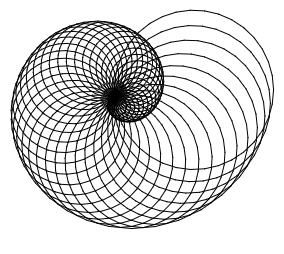
\includegraphics[keepaspectratio, width=\textwidth]{GrundlagenInfo/00_Programmieren/Figures/spirale.png}
\end{figure}
\end{minipage}\\

Leider ist unsere Turtle etwas müde und sollte nicht zu viel laufen. Daher möchten wir fortlaufend die Gesamtdistanz berechnen, um am Ende herauszufinden, ob unsere Turtle zu viel Strecke zurückgelegt hat. Dies können wir tun, indem wir die Funktion einen Wert zurückgeben lassen:
\begin{lstlisting}
from gturtle import *
makeTurtle()
hideTurtle()

def vieleck(umfang, ecken):
    repeat ecken:
        fd(umfang/ecken)
        rt(360/ecken)

def vieleck_muster(umfang, ecken):
	(*@\colorbox{CornflowerBlue}{gesamtdistanz=0}@*)
    while umfang>50:
        vieleck(umfang, ecken)
        (*@\colorbox{CornflowerBlue}{gesamtdistanz+=umfang}@*)
        umfang-=10
        rt(10)
    (*@\colorbox{CornflowerBlue}{return gesamtdistanz}@*)
    
(*@\colorbox{CornflowerBlue}{gesamtdistanz = }@*)vieleck_muster(500,35)
(*@\colorbox{CornflowerBlue}{print(gesamtdistanz)}@*)
\end{lstlisting}


\end{myexample}

Definitionen können zudem Inputs entgegennehmen, sogenannte \textbf{Parameter}. Wir zwar bisher einen Wert einer Variable mittels \lstinline|drucken|, Bisher konnten Sie jedoch nichts an das Hauptprogramm zurückgeben. In diesem Kapitel lernen wir, dass dies möglich ist mit dem Befehl \lstinline|return|.

Eine Funktion kann man sich vorstellen wie ein Kochrezept, das einige Zutaten entgegennimmt und ein Resultat (Gericht) zurückgibt. Die Zutaten, oder ``Inputs'', werden dabei häufig als ``\textbf{Parameter}'' bezeichnet, währenddem das fertige Gericht, oder ``Resultat'' häufig als ``\textbf{\lstinline|return|-Wert}'' bezeichnet wird. Diese Idee ist in \cref{fig:funktion-einzeln}) veranschaulicht.

\begin{figure}[H]
% Use the \drawCube macro to draw various cubes
\centering
\begin{tikzpicture}
\drawCube{1}{0}{2}{3}
\node[fill=blue!50, rounded corners] (input1) at (llD11val){3};
\node[fill=blue!50, rounded corners] (input2) at (llD21val){12};
\draw[thick,->] (input1) -- (in11);
\draw[thick,->] (input2) -- (in12);
\node[fill=green!50, rounded corners](outVal1) at (5,-.6,3){36};
\draw[thick,->] (out1) -- (outVal1);
\end{tikzpicture}
\caption{Illustration einer Funktion mit Inputs (Parametern) und Outputs (\lstinline|return|-Wert)}
\label{fig:funktion-einzeln}
\end{figure}

Wozu dient dies? Nun, stellen Sie sich vor, Sie arbeiten in einer edlen Michelin-Sterne-Küche an einem raffinierten Gericht, in das viele Arbeitsschritte involviert sind. Häufig müssen in solchen Restaurants bis zu 200 Schritte pro Gericht ausgeführt werden. Daher könnte es sinnvoll sein, einzelne Aufgaben, wie beispielsweise die Herstellung der Saucen, an Ihre Sous-Chefs zu delegieren, und eine Person zu bestimmen, die das ganze Gericht zusammenfügt. Häufig werden Funktionen genau mit solchen komplexen Aufgaben im Hinterkopf geschrieben. Diese Idee ist in \cref{fig:funktionen-mehrere} illustriert.

\begin{figure}[H]
% Use the \drawCube macro to draw various cubes
\centering
\begin{tikzpicture}
\drawCube{1}{0}{2}{3}
% feed input values into a1
\node[fill=blue!50, rounded corners] (input1) at (llD11val){3};
\node[fill=blue!50, rounded corners] (input2) at (llD21val){12};
\draw[thick,->] (input1) -- (in11);
\draw[thick,->] (input2) -- (in12);
\node[fill=green!50, rounded corners](outVal1) at (5,-.6,3){36};
\draw[thick,->] (out1) -- (outVal1);
\drawCube{2}{5.25}{3}{3}
\drawCube{3}{10.5}{2}{3}
\draw[thick,->,rounded corners] (out1) -- ++(0,-3.25,0) -- ++(3.15,0,0)node[below]{\lstinline[language=Python,style=TigerJython,basicstyle=\ttfamily]{return out1}} -- ++(4.65,0,0) -- (in31);
\end{tikzpicture}
\caption{Illustration einer Code-Struktur, bei welcher mehrere Funktionen zusammenarbeiten}
\label{fig:funktionen-mehrere}
\end{figure}

In \cref{fig:funktionen-mehrere} haben wir eine Funktion \lstinline|a1|, die zwei Parameter entgegennimmt (\lstinline|x1| und \lstinline|x2|). Mit diesen Parametern macht sie etwas (z.B. die Summe berechnen, ein Quadrat zeichnen oder irgend eine sonstige Aufgabe) und gibt danach einen neuen, berechneten Wert \lstinline|a1| zurück. Dieser kann im Hauptprogramm abgespeichert und an andere Funktionen weitergegeben werden, beispielsweise an die Funktion \lstinline|a3|.

Folgendes Beispiel soll dieses Prinzip konkret veranschaulichen. Stellen Sie sich vor, Sie sind SportlerIn und möchten Ihren Kalorienbedarf berechnen, um sich für auf einen kommenden Wettkampf optimal zu ernähren. Eventuell möchten Sie auch noch etwas ab- oder zunehmen, da Ihre Sportart dies erfordert. Hierzu wollen zunächst Sie Ihren täglichen Kalorienbedarf berechnen. Ihr Kalorienbedarf berechnet sich wie folgt:
\begin{enumerate}
\item Ihr Grundumsatz (englisch \gls{BMR}), d.h., ihr Grundbedarf, falls Sie sich nicht bewegen.
\item Ihr Leistungsumsatz, d.h., zusätzliche Energie, die Sie bei Aktivitäten wie Spazieren, Radfahren, Joggen usw. verbrennen.
\end{enumerate}

Beide Komponenten scheinen schwierig abzuschätzen, Sie möchten jedoch eine erste Einschätzung Ihrer \gls{BMR} haben, indem sie einige bekannte Formeln auf sich selber anwenden und diese vergleichen.

\begin{myexercise}\label{ex:bmr-simple}
Schreiben Sie eine Python-Funktion, um den Grundumsatz anhand der Harris-Benedict-Formel berechnen und geben Sie das Resultat auf der Konsole aus.
\begin{enumerate}
\item Für Männer:
\begin{align*}
\text{BMR} = & 88.362 +\\ 
& (13.397 \times \text{Gewicht in kg}) +\\ 
& (4.799 \times \text{Körpergrösse in cm}) -\\
& (5.677 \times \text{Alter in Jahren})
\end{align*}
\item Für Frauen:
\begin{align*}
\text{BMR} = & 447.593  +\\ 
& (9.247 \times \text{Gewicht in kg}) +\\ 
& (3.098 \times \text{Körpergrösse in cm}) -\\
& (4.330 \times \text{Alter in Jahren})
\end{align*}
\end{enumerate}
\begin{myanswer}
\begin{lstlisting}
def grundumsatz(gewicht, groesse, alter, geschlecht):
    """
    Berechnet den Grundumsatz (BMR) nach der Harris-Benedict-Formel.
    
    Parameter:
    - gewicht: Gewicht in kg
    - groesse: Körpergrösse in cm
    - alter: Alter in Jahren
    - geschlecht: 'mann' oder 'frau'
    
    Rückgabe:
    - BMR: Grundumsatz in Kalorien
    """
    if geschlecht == 'mann':
        bmr = 88.362 + (13.397 * gewicht) + (4.799 * groesse) - (5.677 * alter)
    elif geschlecht == 'frau':
        bmr = 447.593 + (9.247 * gewicht) + (3.098 * groesse) - (4.330 * alter)
    
    print("Der Grundumsatz beträgt:", round(bmr, 2), "Kalorien")

# Beispiel:
gewicht = 75  # kg
groesse = 180  # cm
alter = 30  # jahre
geschlecht = 'mann'

# berechne grundumsatz
grundumsatz(gewicht, groesse, alter, geschlecht)
\end{lstlisting}
\end{myanswer}
\end{myexercise}

Nun möchten wir zum Code, den Sie in \cref{ex:bmr-simple} geschrieben haben, zum Grundumsatz auch noch unsere Aktivitäten hinzufügen, allerdings können wir nun nicht mehr auf die Variable \texttt{bmr} zurückgreifen. Wie können wir das ändern? Indem wir sie an das Programm zurückgeben und speichern. Wichtige Änderungen gegebüber den Lösungs-Code aus \cref{ex:bmr-simple} sind in \colorbox{CornflowerBlue}{blau} umrandet.

\begin{minipage}{\linewidth}
\begin{lstlisting}
def grundumsatz(gewicht, groesse, alter, geschlecht):
    if geschlecht == 'mann':
        bmr = 88.362 + (13.397 * gewicht) + (4.799 * groesse) - (5.677 * alter)
    elif geschlecht == 'frau':
        bmr = 447.593 + (9.247 * gewicht) + (3.098 * groesse) - (4.330 * alter)
    
     (*@\colorbox{CornflowerBlue}{return b\tikzmark{arrowFrom}mr}@*) # gib den bmr an das Programm zurück

# Beispiel:
gewicht = 75  # kg
groesse = 180  # cm
alter = 30  # jahre
geschlecht = 'mann'

# berechne grundumsatz(*@\colorbox{CornflowerBlue}{und speichere das Resultat in einer neuen Variable resultat}@*)
(*@\colorbox{CornflowerBlue}{resu\tikzmark{arrowTo}ltat = }@*) grundumsatz(gewicht, groesse, alter, geschlecht)
(*@\colorbox{CornflowerBlue}{print("Der Grundumsatz beträgt:", round(resultat, 2), "Kalorien")}@*)
\end{lstlisting}
\end{minipage}

\begin{tikzpicture}[overlay,remember picture]
   % Wert zurückgeben
	\draw[red,-stealth] (arrowFrom.north) to[bend left] node[right, fill=RoyalBlue,text=white,rounded corners] {Wert Zurückgeben} (arrowTo);
\end{tikzpicture}

Nun haben wir eine erste Einschätzung des \gls{BMR}. Allerdings gibt es auch noch weitere Formeln, die wir gerne berechnen möchten, um einen Vergleich der verschiedenen Methoden zu erhalten.

\begin{mysubmission}\label{ex:bmr}
Schreiben Sie eine weitere Definitionen, um den \gls{BMR} anhand der Mifflin-St-Jeor-Gleichung und der Katch-McArdle-Formel zurückzugeben und berechnen Sie den Durchschnitt aller drei Formeln.
\begin{enumerate}
\item Mifflin-St-Jeor-Gleichung:
\begin{enumerate}
\item Männer: 
\begin{align*}
\text{BMR} &= 10 \times \text{Gewicht (kg)} \\
&\quad + 6.25 \times \text{Größe (cm)} \\
&\quad - 5 \times \text{Alter (Jahre)} \\
&\quad + 5
\end{align*}
\item Frauen: 
\begin{align*}
\text{BMR} &= 10 \times \text{Gewicht (kg)} \\
&\quad + 6.25 \times \text{Größe (cm)} \\
&\quad - 5 \times \text{Alter (Jahre)} \\
&\quad - 161
\end{align*}
\end{enumerate}
\item Katch-McArdle-Formel:
\begin{enumerate}
\item Grundformel:
\begin{align*}
\text{BMR} &= 370 \\
&\quad + (21.6 \times \text{FFM in kg})
\end{align*}

\item Fett-freie Masse (in kg): 
\begin{align*}
\text{FFM} &= \text{Körpergewicht (kg)} \\
&\quad \times (1 - \text{Körperfettanteil})
\end{align*}

\end{enumerate}

\end{enumerate}

\begin{myanswer}
\lstinputlisting{GrundlagenInfo/00_Programmieren/Python/bmr_functions/bmr.py}
\end{myanswer}
\end{mysubmission}

Nun haben wir eine etwas verlässlichere Einschätzung unseres Grundbedarfs. Zu diesem können wir nun auch noch die Leistungsenergie hinzufügen, um den gesamten Energiebedarf zu berechnen.

\begin{mysubmission}\label{ex:leistungsumsatz}
Berechnen Sie Ihre Leistungsenergie anhand der Tabelle \ref{tab:kcal}, indem Sie für zwei Listen erstellen: 
\begin{enumerate}
\item Eine Liste für die Zeit, während der Sie täglich einer Aktivität nachgehen
\item Eine Liste mit dem Kalorienverbrauch pro Minute für jede dieser Aktivitäten
\end{enumerate} 

\begin{table}[H]
\centering
\begin{tabular}{c|*{10}{c}}
\textbf{Gewicht (kg)} & 60 & 65 & 70 & 75 & 80 & 85 & 90 & 95 & 100 & 105 \\
\midrule\midrule
\textbf{Spazieren} & 4.5 & 5.1 & 5.4 & 5.7 & 6.0 & 6.4 & 6.7 & 7.3 & 8.0 & 9.0 \\
\midrule
\textbf{Schnelles Gehen} & 5.5 & 6.3 & 7.0 & 7.5 & 8.0 & 8.6 & 9.5 & 10.0 & 10.6 & 11.3 \\
\midrule
\textbf{Fahrradfahren} & 6.5 & 7.5 & 8.0 & 9.0 & 9.5 & 10.3 & 11.0 & 11.7 & 12.5 & 13.6 \\
\midrule
\textbf{Schwimmen} & 8.0 & 9.2 & 10.0 & 10.8 & 11.5 & 12.5 & 13.7 & 14.4 & 15.4 & 16.5 \\
\midrule
\textbf{Rudern} & 11.0 & 13.0 & 14.3 & 15.0 & 16.5 & 17.5 & 19.0 & 20.5 & 21.8 & 23.5 \\
\midrule
\textbf{Jogging} & 13.0 & 14.5 & 16.0 & 17.5 & 19.0 & 20.0 & 22.0 & 23.5 & 24.5 & 26.5 \\
\midrule
\textbf{Laufen} & 16.0 & 18.5 & 20.0 & 22.0 & 23.5 & 25.0 & 27.5 & 29.0 & 31.0 & 33.5 \\
\midrule
\textbf{Sprint} & 19.0 & 21.5 & 24.0 & 26.0 & 28.0 & 30.0 & 32.5 & 34.7 & 35.6 & 39.0 \\
\end{tabular}
\caption{Kalorienverbrauch für unterschiedliche Aktivitäten, pro Minute}
\label{tab:kcal}
\end{table}
Wenn z.B. eine 80 kg schwere Person 1 Stunde lang rudert und 20 Minuten spaziert wären die Listen wie folgt:
\begin{lstlisting}
l_zeit = [60, 20] # Zeit in Minuten
l_kcal = [16.5, 6] # Kalorien pro Aktivität
\end{lstlisting}
Schreiben Sie eine Python-Funktion \lstinline|berechne_leistungsumsatz|, um Ihren Leistungsumsatz zu berechnen. Das erwartete Resultat für das Beispiel hier wäre: \lstinline|1110| (= Summe von \lstinline|[990, 120]|). Das Resultat soll an das Hauptprogramm zurückgegeben und in einer Variable \texttt{kalorienverbrauch} gespeichert werden.
\begin{myanswer}
\lstinputlisting{GrundlagenInfo/00_Programmieren/Python/bmr_functions/leistungsumsatz.py}
\end{myanswer}

\end{mysubmission}

\begin{mysubmission}
Schreiben Sie nun eine weitere Funktion, die Ihren gesamten Energieumsatz berechnet, als Summe Ihres BMRs, den Sie in \cref{ex:bmr} berechnet haben und Ihres Leistungsumsatzes, den Sie in \cref{ex:leistungsumsatz} berechnet haben.
\end{mysubmission}

\begin{myexercise}
Schreiben Sie eine weitere Definition, die Ihren \gls{BMR} sowie alle Aktivitätsenergien summiert und zurückgibt.
\end{myexercise}

\section{DL \themycounter: Koordinaten \& Zufallszahlen}
\begin{myExBox}[title=DL \themycounter]
\tcbsubtitle{Thema}
Die SuS beschäftigen sich mit der Integration von neuen Python-Modulen, spezifisch sollen Sie sich mit dem \lstinline|random|-Modul. Dabei vertiefen sie ihre Kenntnisse zu Befehlen mit Parametern. Als Resultat generieren sie Zufallsbilder mit \lstinline|turtle| und können Koordinaten der \lstinline|turtle| ablesen und verändern.


\tcbsubtitle{Operationalisierte Lernziele}
\begin{todolist}
    \item Die SuS können in eignen Worten die Bedeutung von \lstinline|from ... import ...| oder \lstinline|from ... import *| erklären und Module wie \lstinline|random| selbständig in ihren Programmen integrieren.
    \item Die SuS können den Befehl \lstinline|x=random.randint(start, end)|, um Zufallszahlen zu generieren, in ein Programm einbauen und sinnvoll verwenden.
    \item Die SuS können das Ergebnis eines vorgegebenes Programm mit \lstinline|turtle|-Befehlen (z.B. \lstinline|forward()|), von Hand in einem Koordinatensystem einzeichnen und dadurch die Position der \lstinline|turtle| am Ende des Programms bestimmen.
    \item Die SuS können die Position der \lstinline|turtle| mithilfe folgender Funktionen verändern und mit \lstinline|print(pos())| wiedergeben: \lstinline|setX(), setY(), setPos(), setheading()|. 
    \item Die SuS können mithilfe von \lstinline|turtle|- und \lstinline|random|-Befehlen, bzw. -Funktionen eigene Befehle, bzw. eigene Funktionen schreiben (mit oder ohne Parameter), die beim Aufrufen Zufallsbilder generieren. In ihren Befehlen sollten mindestens eine Schleife, ein \lstinline|random|-Befehl, eine \lstinline|turtle|-Farbänderung und eine Verzweigung vorkommen.
\end{todolist}

\tcbsubtitle{Grober Lektionsablauf}
\textbf{Lektion 1/2: Module und Koordinaten}

Zu Beginn eine kurze Erklärung zu Modulen in Python mit Bezug auf die vorherigen Lektionen (vordefinierte und neue Befehle). Anschliessend sollen die SuS sich mit dem \lstinline|random|-Modul vertraut machen indem sie eigene Befehle schreiben, welche Befehle des \lstinline|random|-Moduls beinhalten. Zudem sollen sie sich mit dem Prinzip der Koordinaten vertraut machen, indem sie zuerst von Hand \lstinline|turtle|-Porgramme ausführen und danach in eigenen Programmen die Position der \lstinline|turtle| manipulieren und ablesen.

\textbf{Lektion 2/2: Zufallsbild}

In der zweiten Lektion sollen Sie den Inhalt der ersten Lektion nutzen, um eine Funktion (ohne \lstinline|return|), zu schreiben, die nach dem Aufrufen ein zufällig generiertes Bild erzeugt.


\begin{myExBox}[title=Mögliche Schwierigkeiten \& geeignete Massnahmen]
\begin{enumerate}
    \item Die SuS könnten möglicherweise vergessen, dass Befehle sequentiell abgearbeitet werden und könnten daher versuchen, neue Module am Ende des Programms einzufügen. Daher sollte man zu Beginn der DL nochmals erwähnen, dass der Code sequentiell abgearbeitet wird.
    \item Den SuS alle Funktionen eines Moduls zu präsentieren oder Sie die Online-Dokumentationen (bspw. \href{https://docs.python.org/3/library/random.html}{\lstinline|random|-Dokumentation}) durchlesen zu lassen, wäre für sie vermutlich ein  ``\textit{overkill}''. Stattdessen wollte Spickzettel mit den wichtigsten Funktionen angefertigt werden, welchen sie im Unterricht verwenden sollen, sowie einer Kurzbeschreibung zu den jeweiligen Funktionen. Die Beschreibung sollte folgende Punkte beinhalten: Wozu ist die Funktion nützlich? Wie viele Parameter muss man mitgeben? Welche Datentypen müssen die mitgegebenen Parameter haben? Eventuell kann man den SuS zunächst ein paar Beispiel-Codes geben, die sie auf ihre Funktionalität untersuchen sollen. Somit können sie sich beim Schreiben eines eigenen Befehls, an diesen Beispielen orientieren.
\end{enumerate}
\end{myExBox}
\end{myExBox}
\newpage\stepcounter{mycounter}

\section{DL \themycounter: Listen}
\begin{myExBox}[title=DL \themycounter]
\tcbsubtitle{Thema}
In dieser Lektion geht es um das Erstellen, Bearbeiten und Lesen von Listen.

\tcbsubtitle{Operationalisierte Lernziele}
\begin{todolist}
    \item Die SuS können in eignen Worten beschreiben was eine Liste und ein Index sind und deren Bedeutung anhand eines eignen Beispiels veranschaulichen.
    \item Die SuS können in Python eine Liste mit mehreren Werten erstellen, die Werte verändern, einen beliebigen Werte aus der Liste einer neuen Variable übergeben und einen Bereich von Indizes mit \lstinline| [*:*]| angeben, um einen Teil der Liste auszugeben.
    \item Die SuS können mithilfe von \lstinline|.append()| oder \lstinline|.insert()| neue Elemente einer Liste hinzufügen.
    \item Die SuS können mithilfe einer \lstinline|for|-  Schleife die Elemente einer Liste mit Zahlen oder Tupeln von Zahlen durchlaufen und diese Daten nutzen, um die Position der \lstinline|turtle| zu verändern.
\end{todolist}

\tcbsubtitle{Grober Lektionsablauf}
\textbf{Lektion 1/2: Listen}

In der ersten Lektion wird zunächst das Konzept einer Liste eingeführt und mit Beispielen veranschaulicht. Anschliessend sollen die SuS unterschiedliche Übungen zu den Listen lösen, wobei sie zunächst Beispiele analysieren und anschliessend eigene Listen schreiben und deren Elemente mit \lstinline| print()| ausgeben. Danach sollen sie Zufalls-listen erstellen, deren Inhalt sie wiederum mit einer \lstinline|for|-Schliefe ausgeben sollen.

\textbf{Lektion 2/2: Random \lstinline|turtle|}

In der zweiten Lektion sollen sie den Code aus der vorherigen Lektion anpassen, indem Sie Listen einbauen. Ziel ist es, dass Sie am Ende der Lektion ein Programm haben, dass ihnen eine oder mehrere Listen mit zufällige Zahlen oder Koordinaten erstellt, die wiederum genutzt werden, um ein Zufallsbild zu generieren (bspw. ein Blumenfeld).

\begin{myExBox}[title=Mögliche Schwierigkeiten \& geeignete Massnahmen]
\begin{enumerate}
    \item SuS könnten zunächst die Vorstellung haben, dass eine Liste mit dem Index ``1'' beginnt und somit versuchen, dass erste Element einer Liste mit \lstinline|mylist[1]| abzufragen. Eine graphische Darstellung, wobei die Indizes direkt unter der Liste angegeben sind, kann hier weiterhelfen.
    \item Der Unterschied zwischen \lstinline|.append()| und \lstinline|.insert()| könnte möglicherweise unklar sein. Da die SuS bisher nie mit Objekten arbeiten mussten, könnte es zunächst verwirrend sein, warum man den Befehl mit einem Punkt ausführt (z.B. \lstinline|mylist.append("hallo")|). Sie könnten versuchen die Funktion alleinstehend (\lstinline|.append("hallo")|) oder mit der Liste als Parameter \lstinline|.append("hallo", mylist)| aufzurufen. Auch hier kann es nützlich sein einen Spickzettel mit den wichtigsten Informationen (Anzahl Parameter, Parametertypen, Nutzen usw.) anzufertigen und ihnen Beispiele zu geben, die sie analysieren sollen und die ihnen aufzuzeigen, wie man die Funktionen einsetzen könnte.
    \item Ein weiteres Problem könnte die Verschachtelung von Befehlen darstellen: Bspw. \lstinline|mylist.append(randint(1,2))| Hier könnte man den SuS als Tipp mitgeben, damit es für sie übersichtlicher ist, mit Variablen zu arbeiten, bspw. \lstinline|a = randint(1,2)| und dann \lstinline|mylist.append(a)| zu schreiben.
\end{enumerate}
\end{myExBox}
\end{myExBox}


%\newcounter{step}
%\setcounter{step}{0}
%\newcommand{\includesteps}[1]{%
%  \forloop{step}{0}{\value{step} < #1}{%
%    \input{GrundlagenInfo/00_Programmieren/Python/step_\arabic{step}.tex}
%    \clearpage
%  }
%}

% Replace <number_of_steps>tete with the actual number of steps generated
%\includesteps{16}
\begin{figure}[H]
	\include{GrundlagenInfo/00_Programmieren/Python/binary_search_bubble_sort/step_2.tex}	
\end{figure}


